\begin{frame}
\frametitle{Resultados}

\begin{itemize}
\item Imagens de folhas do repositório ImageCLEF (2011) \cite{imageclef2011};
\item Curvas em $\mathbb{R}^2$ e $\mathbb{R}^3$;
\item Malhas poligonais.
\end{itemize}
	
\end{frame}


\begin{frame}
\frametitle{Resultados}

\destaq{Cálculo do erro (distância euclidiana):}

\bigskip
Para cada vértice $i$, o erro dos pontos obtidos $\mathbf{v'}$ em relação aos pontos originais $\mathbf{v}$ é:

$$E_i(\mathbf{v, v'}) = \sqrt{(\mathbf v_i^{(x)} - \mathbf v_i'^{(x)})^2 + (\mathbf v_i^{(y)} - \mathbf v_i'^{(y)})^2}$$

\medskip

\noindent e o erro total da reconstrução é calculado como a soma do erro para cada ponto:

$$E(\mathbf{v, v'}) = \sum_{i = 1}^{|V|}E_i(\mathbf{v, v'})$$

\end{frame}


\begin{frame}
\frametitle{Resultados}
\framesubtitle{Imagens do banco de dados ImageCLEF (2011) \cite{imageclef2011}}
\begin{figure}[ht!]
	\centering
	\caption{Reconstrução em imagens de folhas.}
	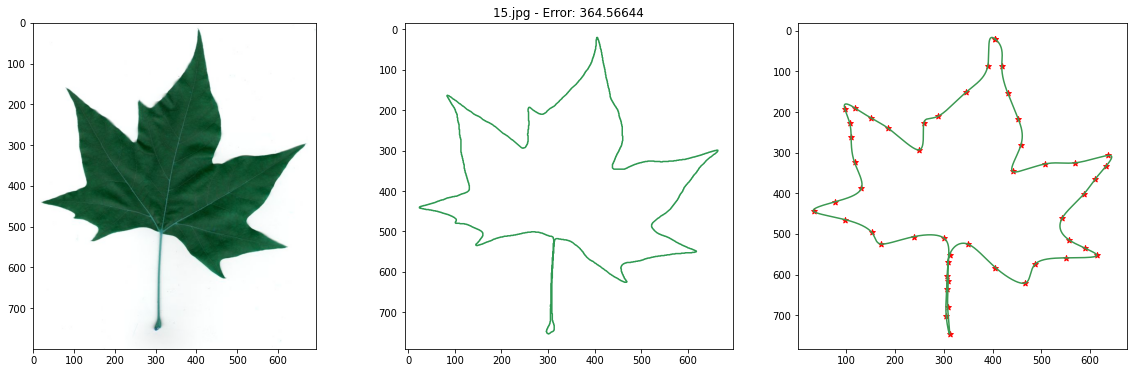
\includegraphics[width=0.9\linewidth]{img/leaf_1.png}
	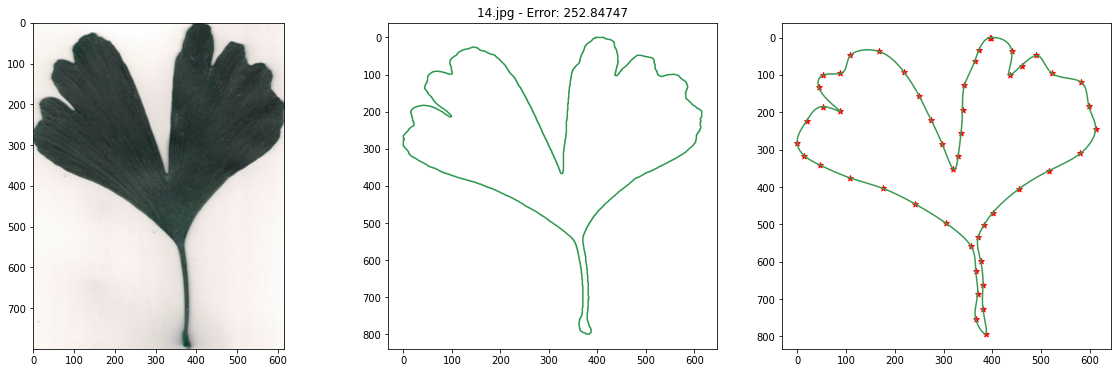
\includegraphics[width=0.9\linewidth]{img/leaf_2.png}
	\label{fig:leafs}
\end{figure}

\end{frame}


\begin{frame}
\frametitle{Resultados}
\framesubtitle{Curvas em $\mathbb{R}^2$ e $\mathbb{R}^3$}

\begin{figure}
	\centering
	\begin{subfigure}[b]{0.31\textwidth}
		\centering
		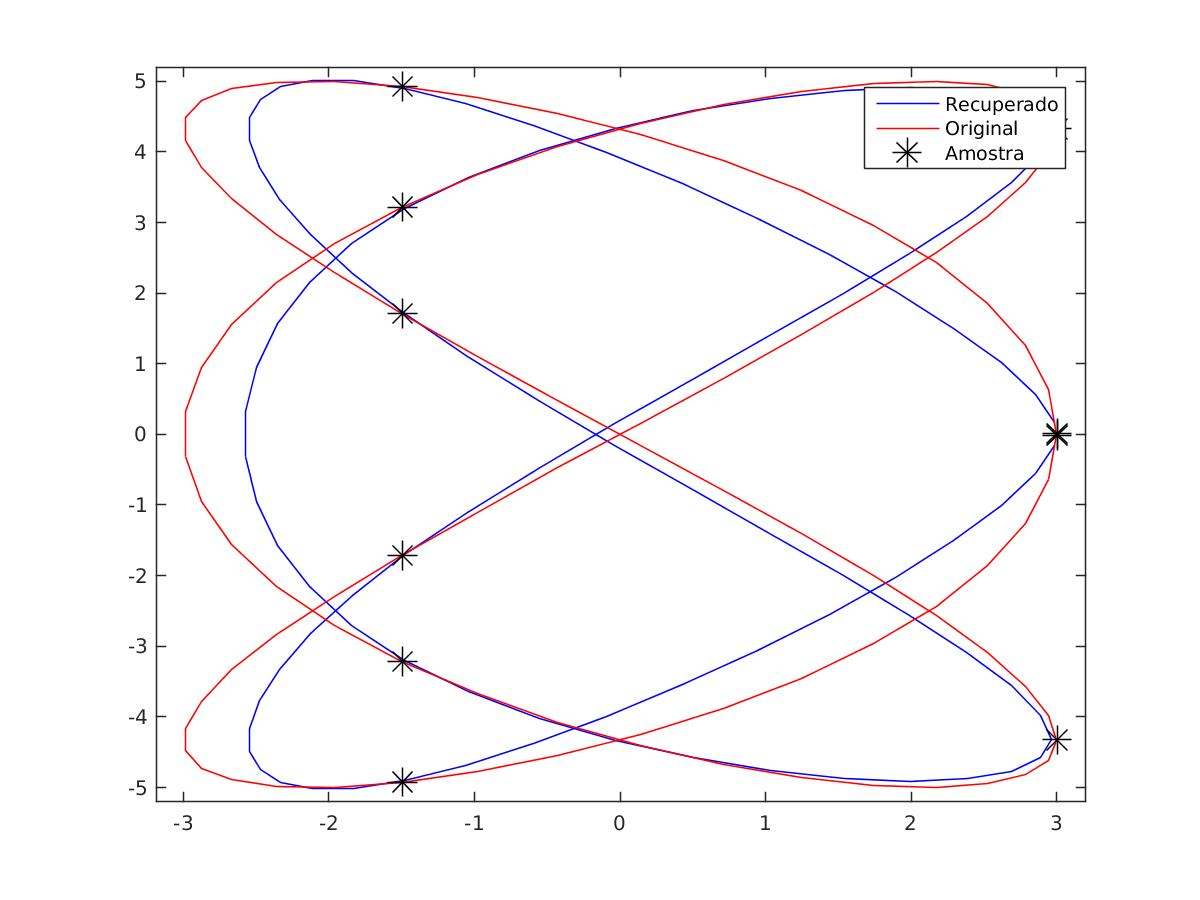
\includegraphics[trim={5cm 2cm 3cm 2cm},clip,width=\textwidth]{img/rep_2_10.jpg}
		\caption{10 pontos}
		\label{fig:ex24}
	\end{subfigure}
	\hfill
	\begin{subfigure}[b]{0.31\textwidth}
		\centering
		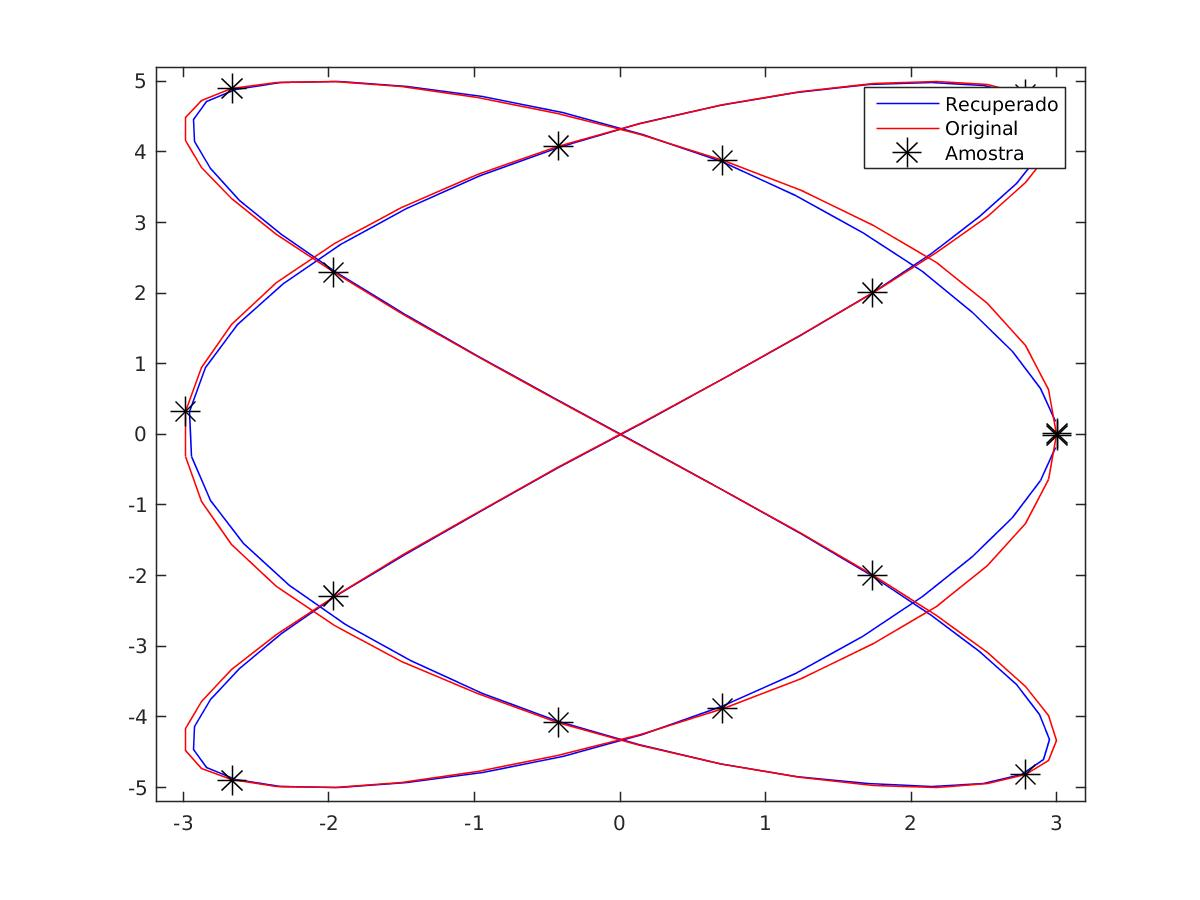
\includegraphics[trim={5cm 2cm 3cm 2cm},clip,width=\textwidth]{img/rep_2_15.jpg}
		\caption{15 pontos}
		\label{fig:ex22}
	\end{subfigure}
	\hfill
	\begin{subfigure}[b]{0.31\textwidth}
		\centering
		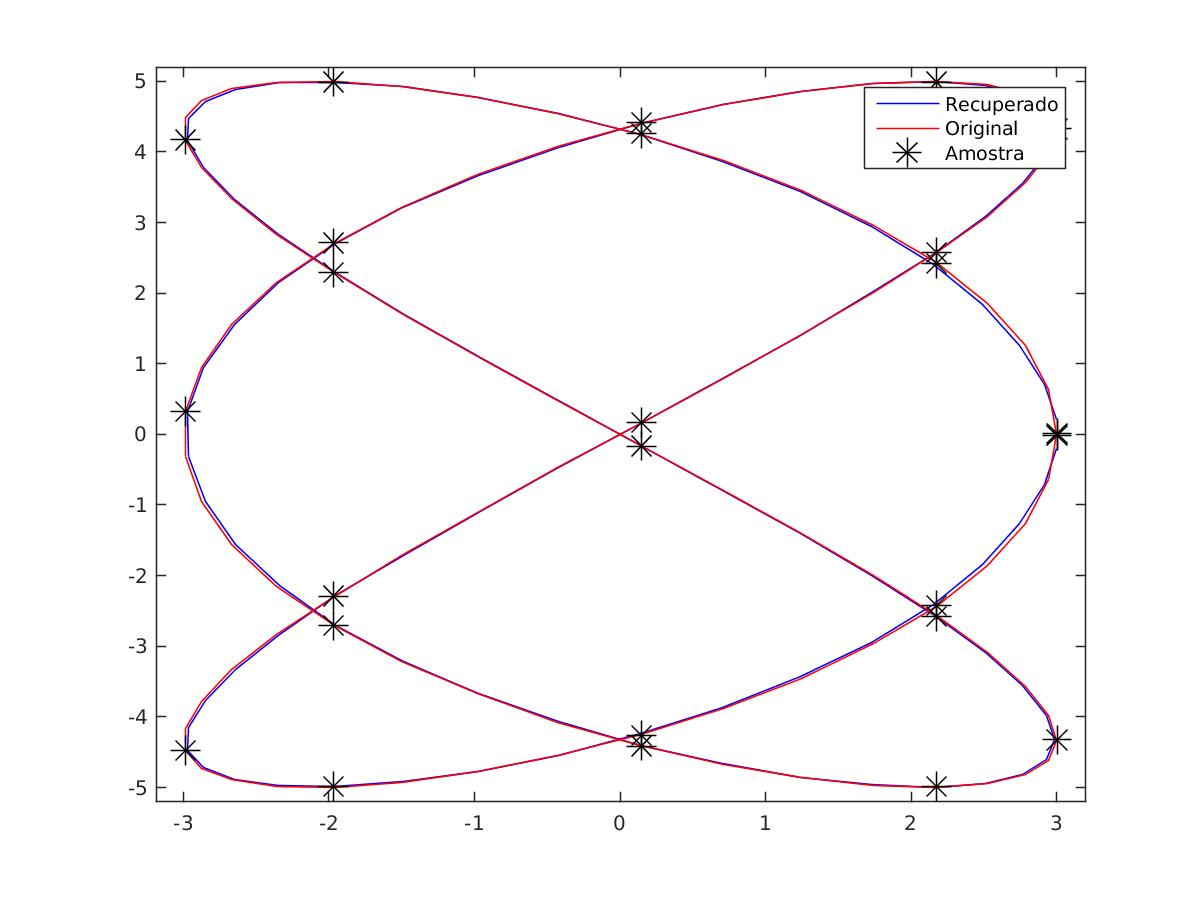
\includegraphics[trim={5cm 2cm 3cm 2cm},clip,width=\textwidth]{img/rep_2_25.jpg}
		\caption{25 pontos}
		\label{fig:ex23}
	\end{subfigure} %[3 * cos(3 * t); 5 * sin(2 * t)]';
	\caption{Representação da função paramétrica $(x(t), y(t)) = (3 cos(3t), 5sen(2t))$ utilizando alguns pontos igualmente espaçados como amostra.}
	\label{fig:ex2rep}
\end{figure}

\end{frame}


\begin{frame}
\frametitle{Resultados}
\framesubtitle{Malhas 3D}

\begin{figure}[hbt]
\begin{center}
	\caption{Representação da malha de um coelho}
	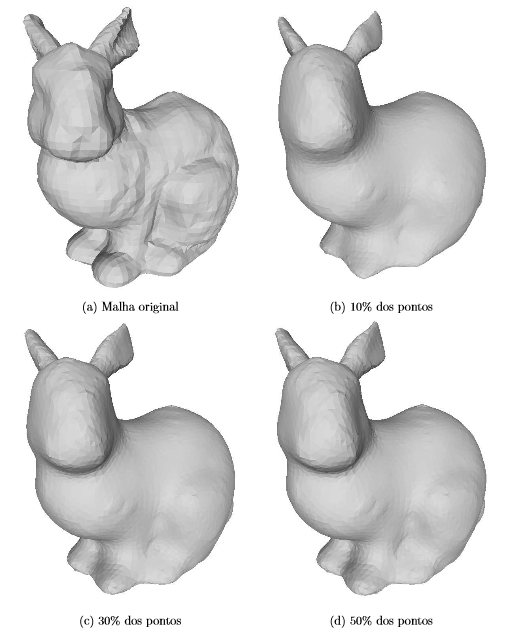
\includegraphics[width=0.45\textwidth]{img/mesh.png}
\end{center}
\end{figure}

\end{frame}


